\documentclass[11pt,a4paper]{article}
\usepackage[a4paper,margin=2.3cm]{geometry}
\usepackage[T1]{fontenc}
\usepackage{newtxtext,newtxmath}
\usepackage{microtype}
\usepackage{booktabs}
\usepackage{graphicx}
\usepackage{amsmath}
\usepackage{xcolor}
\usepackage[colorlinks=true,linkcolor=black,citecolor=black,urlcolor=blue!50!black]{hyperref}
\usepackage{caption}
\captionsetup{font=small,labelfont=bf}
\graphicspath{{../results/figures/}}
% generated by src/make_numbers.py -- do not edit
\newcommand{\DKaacimax}{90.3}
\newcommand{\DKaacimin}{89.5}
\newcommand{\DKabDays}{928}
\newcommand{\DKabFirst}{2024-02-02}
\newcommand{\DKabLast}{2026-09-29}
\newcommand{\DKabRedCvar}{24.4}
\newcommand{\DKabRedCvarOne}{22.9}
\newcommand{\DKabRedDiur}{6.6}
\newcommand{\DKabRedGbm}{22.9}
\newcommand{\DKabRedOracle}{39.6}
\newcommand{\DKabRedQr}{24.7}
\newcommand{\DKabRedRls}{25.9}
\newcommand{\DKabRedScen}{25.2}
\newcommand{\DKabRegCvarCvar}{250}
\newcommand{\DKabRegCvarCvarOne}{258}
\newcommand{\DKabRegCvarDiur}{551}
\newcommand{\DKabRegCvarGbm}{283}
\newcommand{\DKabRegCvarOracle}{0}
\newcommand{\DKabRegCvarQr}{266}
\newcommand{\DKabRegCvarRls}{254}
\newcommand{\DKabRegCvarScen}{263}
\newcommand{\DKabRegMeanCvar}{88}
\newcommand{\DKabRegMeanCvarOne}{96}
\newcommand{\DKabRegMeanDiur}{191}
\newcommand{\DKabRegMeanGbm}{96}
\newcommand{\DKabRegMeanOracle}{0}
\newcommand{\DKabRegMeanQr}{86}
\newcommand{\DKabRegMeanRls}{79}
\newcommand{\DKabRegMeanScen}{83}
\newcommand{\DKabRegPnfCvar}{227}
\newcommand{\DKabRegPnfCvarOne}{242}
\newcommand{\DKabRegPnfDiur}{521}
\newcommand{\DKabRegPnfGbm}{265}
\newcommand{\DKabRegPnfOracle}{0}
\newcommand{\DKabRegPnfQr}{243}
\newcommand{\DKabRegPnfRls}{228}
\newcommand{\DKabRegPnfScen}{242}
\newcommand{\DKabShareCvar}{62}
\newcommand{\DKabShareCvarOne}{58}
\newcommand{\DKabShareDiur}{17}
\newcommand{\DKabShareGbm}{58}
\newcommand{\DKabShareOracle}{100}
\newcommand{\DKabShareQr}{62}
\newcommand{\DKabShareRls}{65}
\newcommand{\DKabShareScen}{64}
\newcommand{\DKacDays}{959}
\newcommand{\DKacDaysShortFive}{100}
\newcommand{\DKacDaysShortOne}{100}
\newcommand{\DKacDaysShortTen}{100}
\newcommand{\DKacDaysShortTwo}{100}
\newcommand{\DKacOptFive}{0.9}
\newcommand{\DKacOptOne}{1.3}
\newcommand{\DKacOptTen}{0.8}
\newcommand{\DKacOptTwo}{1.1}
\newcommand{\DKacShortFive}{7.2}
\newcommand{\DKacShortMaxFive}{11.2}
\newcommand{\DKacShortMaxOne}{13.4}
\newcommand{\DKacShortMaxTen}{9.7}
\newcommand{\DKacShortMaxTwo}{12.1}
\newcommand{\DKacShortOne}{7.6}
\newcommand{\DKacShortTen}{6.6}
\newcommand{\DKacShortTwo}{7.7}
\newcommand{\DKacopCorr}{0.38}
\newcommand{\DKacovEightyAci}{79.6}
\newcommand{\DKacovEightyGauss}{79.9}
\newcommand{\DKacovEightyQr}{78.9}
\newcommand{\DKacovNinetyAci}{90.0}
\newcommand{\DKacovNinetyGauss}{89.4}
\newcommand{\DKacovNinetyQr}{88.5}
\newcommand{\DKadaMaeDiur}{47.9}
\newcommand{\DKadaMaeGbm}{29.3}
\newcommand{\DKadaMaeProg}{5.6}
\newcommand{\DKadaMaeRls}{27.5}
\newcommand{\DKadaRed}{43}
\newcommand{\DKadaRedGbm}{39}
\newcommand{\DKadaRmseDiur}{62.3}
\newcommand{\DKadaRmseGbm}{37.9}
\newcommand{\DKadaRmseProg}{9.4}
\newcommand{\DKadaRmseRls}{34.9}
\newcommand{\DKadmDiurP}{<10^{-4}}
\newcommand{\DKadmDiurStat}{25.1}
\newcommand{\DKadmGbmP}{<10^{-4}}
\newcommand{\DKadmGbmStat}{4.2}
\newcommand{\DKaflagged}{2}
\newcommand{\DKalamDA}{0.99}
\newcommand{\DKalamST}{0.995}
\newcommand{\DKameanY}{97.6}
\newcommand{\DKaqsGauss}{9.39}
\newcommand{\DKaqsQr}{9.60}
\newcommand{\DKastGbmOne}{12.3}
\newcommand{\DKastGbmSix}{24.6}
\newcommand{\DKastGbmTwelve}{25.8}
\newcommand{\DKastPersOne}{13.4}
\newcommand{\DKastPersSix}{37.4}
\newcommand{\DKastPersTwelve}{45.0}
\newcommand{\DKastRedTwelve}{42}
\newcommand{\DKastRlsOne}{12.9}
\newcommand{\DKastRlsSix}{25.1}
\newcommand{\DKastRlsTwelve}{26.2}
\newcommand{\DKatopAci}{92.3}
\newcommand{\DKatopGauss}{85.2}
\newcommand{\DKatopQr}{91.4}
\newcommand{\DKawidthEightyAci}{92}
\newcommand{\DKawidthEightyGauss}{89}
\newcommand{\DKawidthEightyQr}{91}
\newcommand{\DKawidthNinetyAci}{120}
\newcommand{\DKawidthNinetyGauss}{114}
\newcommand{\DKawidthNinetyQr}{115}
\newcommand{\DKbacimax}{93.9}
\newcommand{\DKbacimin}{86.9}
\newcommand{\DKbbDays}{924}
\newcommand{\DKbbFirst}{2024-02-02}
\newcommand{\DKbbLast}{2026-09-29}
\newcommand{\DKbbRedCvar}{21.7}
\newcommand{\DKbbRedCvarOne}{20.7}
\newcommand{\DKbbRedDiur}{6.5}
\newcommand{\DKbbRedGbm}{23.1}
\newcommand{\DKbbRedOracle}{34.6}
\newcommand{\DKbbRedQr}{22.9}
\newcommand{\DKbbRedRls}{23.4}
\newcommand{\DKbbRedScen}{23.0}
\newcommand{\DKbbRegCvarCvar}{164}
\newcommand{\DKbbRegCvarCvarOne}{170}
\newcommand{\DKbbRegCvarDiur}{397}
\newcommand{\DKbbRegCvarGbm}{176}
\newcommand{\DKbbRegCvarOracle}{0}
\newcommand{\DKbbRegCvarQr}{176}
\newcommand{\DKbbRegCvarRls}{159}
\newcommand{\DKbbRegCvarScen}{170}
\newcommand{\DKbbRegMeanCvar}{47}
\newcommand{\DKbbRegMeanCvarOne}{51}
\newcommand{\DKbbRegMeanDiur}{103}
\newcommand{\DKbbRegMeanGbm}{42}
\newcommand{\DKbbRegMeanOracle}{0}
\newcommand{\DKbbRegMeanQr}{43}
\newcommand{\DKbbRegMeanRls}{41}
\newcommand{\DKbbRegMeanScen}{43}
\newcommand{\DKbbRegPnfCvar}{137}
\newcommand{\DKbbRegPnfCvarOne}{149}
\newcommand{\DKbbRegPnfDiur}{381}
\newcommand{\DKbbRegPnfGbm}{157}
\newcommand{\DKbbRegPnfOracle}{0}
\newcommand{\DKbbRegPnfQr}{158}
\newcommand{\DKbbRegPnfRls}{140}
\newcommand{\DKbbRegPnfScen}{145}
\newcommand{\DKbbShareCvar}{63}
\newcommand{\DKbbShareCvarOne}{60}
\newcommand{\DKbbShareDiur}{19}
\newcommand{\DKbbShareGbm}{67}
\newcommand{\DKbbShareOracle}{100}
\newcommand{\DKbbShareQr}{66}
\newcommand{\DKbbShareRls}{67}
\newcommand{\DKbbShareScen}{66}
\newcommand{\DKbcDays}{955}
\newcommand{\DKbcDaysShortFive}{100}
\newcommand{\DKbcDaysShortOne}{100}
\newcommand{\DKbcDaysShortTen}{100}
\newcommand{\DKbcDaysShortTwo}{100}
\newcommand{\DKbcOptFive}{1.2}
\newcommand{\DKbcOptOne}{1.6}
\newcommand{\DKbcOptTen}{1.0}
\newcommand{\DKbcOptTwo}{1.5}
\newcommand{\DKbcShortFive}{7.2}
\newcommand{\DKbcShortMaxFive}{10.4}
\newcommand{\DKbcShortMaxOne}{13.0}
\newcommand{\DKbcShortMaxTen}{9.9}
\newcommand{\DKbcShortMaxTwo}{13.5}
\newcommand{\DKbcShortOne}{7.8}
\newcommand{\DKbcShortTen}{6.9}
\newcommand{\DKbcShortTwo}{7.9}
\newcommand{\DKbcopCorr}{0.34}
\newcommand{\DKbcovEightyAci}{80.8}
\newcommand{\DKbcovEightyGauss}{83.8}
\newcommand{\DKbcovEightyQr}{73.2}
\newcommand{\DKbcovNinetyAci}{90.5}
\newcommand{\DKbcovNinetyGauss}{90.7}
\newcommand{\DKbcovNinetyQr}{83.7}
\newcommand{\DKbdaMaeDiur}{27.3}
\newcommand{\DKbdaMaeGbm}{17.6}
\newcommand{\DKbdaMaeProg}{4.4}
\newcommand{\DKbdaMaeRls}{18.2}
\newcommand{\DKbdaRed}{33}
\newcommand{\DKbdaRedGbm}{35}
\newcommand{\DKbdaRmseDiur}{40.7}
\newcommand{\DKbdaRmseGbm}{26.6}
\newcommand{\DKbdaRmseProg}{6.6}
\newcommand{\DKbdaRmseRls}{25.7}
\newcommand{\DKbdmDiurP}{<10^{-4}}
\newcommand{\DKbdmDiurStat}{14.8}
\newcommand{\DKbdmGbmP}{=0.086}
\newcommand{\DKbdmGbmStat}{-1.7}
\newcommand{\DKbflagged}{4}
\newcommand{\DKblamDA}{0.98}
\newcommand{\DKblamST}{0.998}
\newcommand{\DKbmeanY}{61.9}
\newcommand{\DKbqsGauss}{6.52}
\newcommand{\DKbqsQr}{6.29}
\newcommand{\DKbstGbmOne}{7.6}
\newcommand{\DKbstGbmSix}{14.6}
\newcommand{\DKbstGbmTwelve}{15.2}
\newcommand{\DKbstPersOne}{8.3}
\newcommand{\DKbstPersSix}{24.0}
\newcommand{\DKbstPersTwelve}{29.2}
\newcommand{\DKbstRedTwelve}{41}
\newcommand{\DKbstRlsOne}{8.5}
\newcommand{\DKbstRlsSix}{16.8}
\newcommand{\DKbstRlsTwelve}{17.3}
\newcommand{\DKbtopAci}{91.0}
\newcommand{\DKbtopGauss}{85.5}
\newcommand{\DKbtopQr}{89.4}
\newcommand{\DKbwidthEightyAci}{58}
\newcommand{\DKbwidthEightyGauss}{63}
\newcommand{\DKbwidthEightyQr}{51}
\newcommand{\DKbwidthNinetyAci}{78}
\newcommand{\DKbwidthNinetyGauss}{81}
\newcommand{\DKbwidthNinetyQr}{70}

\newcommand{\gk}{g\,CO$_2$/kWh}

\title{Probabilistic Forecasting of Danish Grid Carbon Intensity\\and Its Value for Flexible Data-Centre Load}
\author{Xiangyu Luo\\\small\href{https://github.com/TeamFan/dk-carbon-intensity-forecasting}{github.com/TeamFan/dk-carbon-intensity-forecasting}}
\date{October 2026}

\begin{document}
\maketitle

\begin{abstract}
\noindent
A flexible load, such as deferrable computing in an edge data centre, can only move its consumption to cleaner hours if those hours are predicted before they happen.
This study forecasts the hourly CO$_2$ intensity of consumed electricity in both Danish bidding zones (DK1, DK2) from Energinet open data, issued every hour for 1--12\,h ahead and once a day for the 24 hours of the next day (9--32\,h ahead), using only inputs that are published before each issue time.
Adaptive ARX models estimated by recursive least squares with exponential forgetting reduce the day-ahead mean absolute error by \DKadaRed\% (DK1) and \DKbdaRed\% (DK2) relative to diurnal persistence over 33 test months (January 2024--September 2026); day-ahead they are more accurate than gradient-boosted trees refitted every month in DK1 and statistically indistinguishable in DK2.
An adaptive Gaussian predictive distribution, a monthly refitted quantile regression and an adaptive conformal correction are compared: the Gaussian intervals are calibrated on average but under-cover the high-intensity hours, and the conformal step brings the empirical coverage of the 90\% day-ahead interval to \DKacovNinetyAci\% (DK1) and \DKbcovNinetyAci\% (DK2).
Used to schedule 6\,MWh of deferrable daily load, the adaptive forecasts capture \DKabShareRls\% (DK1) and \DKbbShareRls\% (DK2) of the emission reduction available with perfect information, against \DKabShareDiur\% and \DKbbShareDiur\% for diurnal persistence; risk-averse CVaR schedules buy a small reduction of tail regret with a larger loss in mean reduction.
Finally, for a fleet of 30 heterogeneous sites, a single aggregate (virtual-battery) envelope leaves \DKacShortOne\% (DK1) of the planned energy undeliverable at site level, which shows that a compact flexibility representation must be checked for disaggregation.
\end{abstract}

\section{Questions}
\begin{enumerate}
\item How accurately can the average CO$_2$ intensity of Danish electricity be forecast from minutes-old measurements and day-ahead market information, and does an adaptive linear model suffice?
\item Are the predictive distributions calibrated across seasons, years and high-intensity hours?
\item How much of the attainable emission reduction of a flexible load is realised when it is scheduled on these forecasts, and does uncertainty information change the schedule?
\item When the flexibility of many sites is summarised by one aggregate model, can the resulting fleet schedule be executed by the individual sites?
\end{enumerate}

\section{Data and information set}
\label{sec:data}
All data are public and were downloaded from Energi Data Service (Energinet) for 1 January 2023 to 30 September 2026, at hourly resolution in UTC (Table~\ref{tab:data}).
The target is the hourly mean of the five-minute series \texttt{CO2Emis}, the average emission intensity of consumed electricity under the 125\% method.
Energinet states that these values come from upscaled real-time measurements and that errors are not corrected; hours with fewer than 9 of 12 values are left missing, and values that are negative or form isolated spikes of more than 100\,\gk{} not shared by Energinet's own schedule-based estimate are removed (\DKaflagged{} hours in DK1 and \DKbflagged{} in DK2, mostly at daylight-saving transitions).

\begin{table}[h]
\centering\small
\caption{Inputs and the time at which they are assumed known.}
\label{tab:data}
\begin{tabular}{@{}p{3.3cm}p{5.4cm}p{6.3cm}@{}}
\toprule
Dataset & Use & Availability assumed\\
\midrule
\texttt{CO2Emis} & target, lags & at the end of each hour (5-min real-time series)\\
\texttt{Forecasts\_Hour} & day-ahead wind (on- and offshore) and solar forecast & for day $D$, before 12:00 UTC on $D-1$\\
\texttt{Elspotprices}, \texttt{DayAheadPrices} & day-ahead price of the zone and of DE, NO2, SE3, SE4 & for day $D$, after the auction around 11:00--12:00 UTC on $D-1$\\
\texttt{CO2EmisProg} & reference only & last intraday update is archived; not a day-ahead forecast\\
\bottomrule
\end{tabular}
\end{table}

\paragraph{Products.}
The \emph{short-term} product is issued every hour $t$ for $t+h$, $h=1,\dots,12$; every input it uses for target hour $t+h$ is available at $t$ under Table~\ref{tab:data}.
The \emph{day-ahead} product is issued after the hour 15:00--16:00 UTC of day $D-1$ for the 24 UTC hours of day $D$ ($h=9,\dots,32$); it is the input to the scheduling study.
Energinet's archived prognosis (\texttt{CO2EmisProg}) is updated from production schedules during the day and only its last update, which can be made shortly before delivery, is stored; its day-ahead MAE of \DKadaMaeProg{} (DK1) and \DKbdaMaeProg{} \gk{} (DK2) therefore reflects intraday information and is reported only as a reference, not as a competing day-ahead forecast.

\paragraph{Split.} The adaptive models start on 1 January 2023; the first half of 2023 is a burn-in period, the second half selects the forgetting factors, and all reported scores are computed on 1 January 2024--30 September 2026.

\section{Methods}
\subsection{Point forecasts}
\paragraph{Benchmarks.} Persistence $\hat y_{t+h|t}=y_t$ (short-term) and diurnal persistence $\hat y_{t+h|t}=y_{t+h-24k}$, $k=\lceil h/24\rceil$, the most recent observation of the same hour (day-ahead).

\paragraph{Adaptive ARX (direct strategy).}
For each horizon (short-term) or target hour (day-ahead) a separate linear model $\hat y_{t+h|t}=x_{t,h}^\top\hat\theta_{h,t}$ is fitted, where $x_{t,h}$ contains an intercept, the latest observations and the diurnal lag, the day-ahead wind, solar and price inputs of the target hour, their changes from the issue hour, harmonics of the hour of day, and the tanh-scaled price spreads to the interconnected zones together with coupling indicators ($|\text{spread}|<0.5$\,EUR/MWh), which indicate whether the marginal supply is shared with a neighbour.
The parameters minimise an exponentially weighted least-squares criterion,
\begin{equation}
\hat\theta_{h,t}=\arg\min_\theta \sum_{s:\,s+h\le t}\lambda^{\,t-s}\bigl(y_{s+h}-x_{s,h}^\top\theta\bigr)^2+\lambda^{t}\delta\|\theta\|^2,
\end{equation}
computed recursively (RLS). A pair $(x_{s,h},y_{s+h})$ enters the estimator only after $y_{s+h}$ has been observed, so no forecast uses information from after its issue time (checked by a unit test that perturbs future targets).
The forgetting factor is chosen on 2023H2 from a small grid: $\lambda=\DKalamST$ / \DKalamDA{} (DK1, short-term / day-ahead) and \DKblamST{} / \DKblamDA{} (DK2), i.e.\ effective memories of roughly 8--21 days for the short-term models and 50--100 days for the day-ahead models.

\paragraph{Non-linear benchmark.} Histogram gradient-boosted trees with absolute-error loss on the same inputs, refitted at the start of every month on the preceding year of resolved pairs.

\subsection{Predictive distributions}
\begin{itemize}
\item \textbf{Gaussian--EWMA.} $\mathcal N(\hat y_{t+h|t},\hat\sigma^2_{h,t})$ with $\hat\sigma^2_{h,t}$ an exponentially weighted mean of past squared errors of the same model.
\item \textbf{Quantile regression (QR).} For $\tau\in\{0.05,0.1,0.2,\dots,0.9,0.95\}$, the linear quantile regression of $y_{t+h}$ on $(1,\hat y_{t+h|t},\text{wind},\text{solar},\text{price})$ minimises the pinball loss with weights $0.995^{\text{age in days}}$ over the preceding year, solved exactly as a linear programme and refitted monthly; crossing quantiles are sorted.
\item \textbf{QR with adaptive conformal inference (ACI)} \cite{gibbs2021}. The central QR interval is widened by the $(1-\alpha_t)$-quantile of recent conformity scores $\max(\hat q_{\mathrm{lo}}-y,\,y-\hat q_{\mathrm{hi}})$, where $\alpha_{t+1}=\alpha_t+\gamma(\alpha-\mathrm{err}_t)$ and $\mathrm{err}_t$ is a miss of an interval whose target has already been observed.
\end{itemize}
Scores: mean absolute error (MAE), root mean squared error, the average quantile (pinball) score QS over the eleven levels, interval coverage and width, and Diebold--Mariano tests on daily mean absolute errors with a Newey--West variance (lag 7).

\subsection{Scheduling a flexible load}
\label{sec:sched}
A site must run $E=6$\,MWh of deferrable computing during day $D$ with at most $P=1$\,MW in any hour; the reference spreads it uniformly.
Given a forecast $c\in\mathbb R^{24}$, the optimal schedule of $\min\{c^\top p:\ \mathbf 1^\top p=E,\ 0\le p\le P\}$ fills the hours with the lowest forecast.
The risk-averse schedule solves
\begin{equation}
\min_{p,\eta,z\ge0}\ (1-\beta)\,\tfrac1S\textstyle\sum_s c_s^\top p+\beta\Bigl(\eta+\tfrac{1}{(1-\alpha)S}\sum_s z_s\Bigr)
\quad\text{s.t.}\ z_s\ge c_s^\top p-\eta,\ \mathbf 1^\top p=E,\ 0\le p\le P,
\end{equation}
the Rockafellar--Uryasev form of the mean--CVaR$_\alpha$ objective \cite{rockafellar2000}, with $\alpha=0.9$ and $S=500$ scenarios drawn from the QR quantiles through a Gaussian copula \cite{pinson2009}; its correlation matrix is estimated from the normal scores of past probability-integral transforms (the 90 most recent days that are already resolved) and shrunk by 10\% towards the identity.
Every schedule is evaluated with the realised intensity; the resulting emissions follow average-intensity (location-based) accounting and are not marginal emission reductions of the power system.

\subsection{Aggregating a fleet}
\label{sec:fleet}
Thirty sites have time windows $[a_i,b_i)$, power caps $P_i$ and daily energies $E_i$ drawn once at random (seed 7).
The exact fleet problem is a joint LP over all site schedules.
A compact aggregate model replaces the sites by one virtual battery with power bound $\sum_{i:\,h\in[a_i,b_i)}P_i$ and cumulative-energy bounds obtained by summing each site's earliest and latest feasible cumulative energy.
This envelope contains every feasible fleet profile but is generally larger than the true set (the Minkowski sum of the site sets).
The aggregate optimum, computed on the day-ahead adaptive forecast, is then split into site schedules by an LP that minimises the site energy left undelivered while never exceeding the aggregate profile.
Grouping the sites into $k$ clusters of similar windows and using one envelope per cluster interpolates between the single envelope ($k=1$) and the exact model ($k=30$).

\section{Results}
\subsection{Point accuracy}
\begin{figure}[t]
\centering
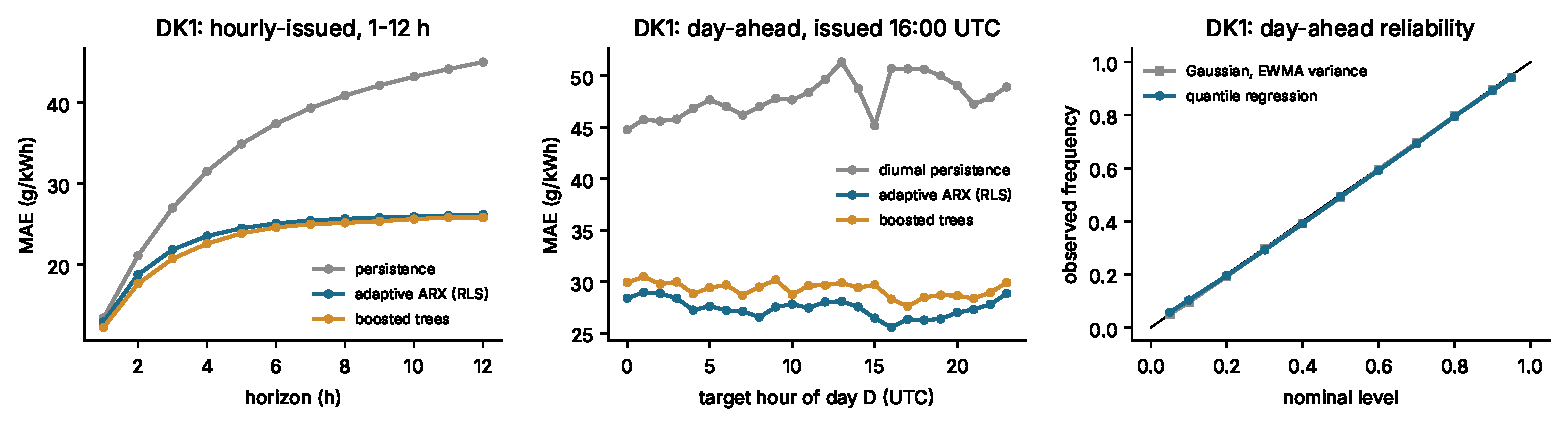
\includegraphics[width=\linewidth]{forecast_skill_DK1.pdf}\\[2pt]
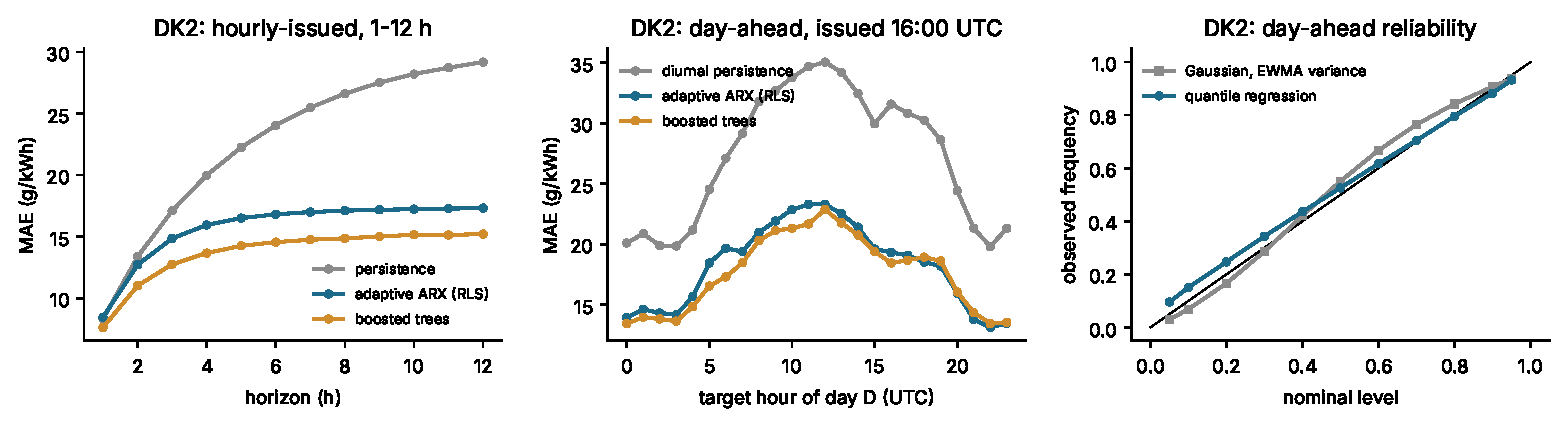
\includegraphics[width=\linewidth]{forecast_skill_DK2.pdf}
\caption{Test-period accuracy (2024-01 to 2026-09). Left: short-term MAE by horizon. Middle: day-ahead MAE by target hour. Right: reliability of the day-ahead predictive quantiles.}
\label{fig:skill}
\end{figure}

Over the test period the mean intensity was \DKameanY{} \gk{} in DK1 and \DKbmeanY{} \gk{} in DK2.
Day-ahead, the adaptive ARX model reaches an MAE of \DKadaMaeRls{} (DK1) and \DKbdaMaeRls{} \gk{} (DK2), against \DKadaMaeDiur{} and \DKbdaMaeDiur{} for diurnal persistence and \DKadaMaeGbm{} and \DKbdaMaeGbm{} for the boosted trees (Figure~\ref{fig:skill}).
The improvement over persistence is significant (Diebold--Mariano statistic \DKadmDiurStat, $p\DKadmDiurP$ in DK1; \DKbdmDiurStat, $p\DKbdmDiurP$ in DK2). Against the trees, the adaptive model is significantly better in DK1 (statistic \DKadmGbmStat, $p\DKadmGbmP$), while in DK2 the difference is not significant (\DKbdmGbmStat, $p\DKbdmGbmP$).
For the short-term product (Table~\ref{tab:st}), persistence is hard to beat at one hour (DK1: \DKastPersOne{} vs \DKastRlsOne; DK2: \DKbstPersOne{} vs \DKbstRlsOne), while at 12 hours the adaptive model is \DKastRedTwelve\% (DK1) and \DKbstRedTwelve\% (DK2) more accurate than persistence.
Here the trees are more accurate than the adaptive linear model at every horizon, most clearly in DK2 (\DKbstGbmTwelve{} vs \DKbstRlsTwelve{} at 12 hours). A plausible explanation is that with hourly issue times they are trained on about 24 times more pairs per horizon than the day-ahead models, enough to exploit non-linear dependence on the latest observations, whereas with one pair per day the adaptive model's ability to follow slow changes matters more.

\begin{table}[h]
\centering\small
\caption{Short-term MAE (\gk) by horizon $h$, test period.}
\label{tab:st}
\begin{tabular}{@{}rccc@{\hspace{1.6em}}ccc@{}}
\toprule
 & \multicolumn{3}{c}{DK1} & \multicolumn{3}{c}{DK2}\\
\cmidrule(lr){2-4}\cmidrule(lr){5-7}
$h$ & persistence & adaptive ARX & trees & persistence & adaptive ARX & trees\\
\midrule
\csname @@input\endcsname tables/st_point.tex 
\bottomrule
\end{tabular}
\end{table}

\subsection{Calibration}
\begin{table}[h]
\centering\small
\caption{Day-ahead predictive distributions, test period: quantile score (QS), coverage and mean width of the central intervals, and coverage of the 90\% interval in the hours whose median forecast lies in the top quintile.}
\label{tab:prob}
\begin{tabular}{@{}lcccccc@{}}
\toprule
& QS & cov.\ 80\% & width 80\% & cov.\ 90\% & width 90\% & cov.\ 90\%, top quintile\\
\midrule
DK1 Gaussian--EWMA & \DKaqsGauss & \DKacovEightyGauss & \DKawidthEightyGauss & \DKacovNinetyGauss & \DKawidthNinetyGauss & \DKatopGauss\\
DK1 QR & \DKaqsQr & \DKacovEightyQr & \DKawidthEightyQr & \DKacovNinetyQr & \DKawidthNinetyQr & \DKatopQr\\
DK1 QR + ACI & -- & \DKacovEightyAci & \DKawidthEightyAci & \DKacovNinetyAci & \DKawidthNinetyAci & \DKatopAci\\
\midrule
DK2 Gaussian--EWMA & \DKbqsGauss & \DKbcovEightyGauss & \DKbwidthEightyGauss & \DKbcovNinetyGauss & \DKbwidthNinetyGauss & \DKbtopGauss\\
DK2 QR & \DKbqsQr & \DKbcovEightyQr & \DKbwidthEightyQr & \DKbcovNinetyQr & \DKbwidthNinetyQr & \DKbtopQr\\
DK2 QR + ACI & -- & \DKbcovEightyAci & \DKbwidthEightyAci & \DKbcovNinetyAci & \DKbwidthNinetyAci & \DKbtopAci\\
\bottomrule
\end{tabular}
\end{table}

Table~\ref{tab:prob} and Figure~\ref{fig:cov} summarise the day-ahead distributions.
The Gaussian--EWMA distribution is calibrated on average (90\% coverage \DKacovNinetyGauss\% in DK1, \DKbcovNinetyGauss\% in DK2) and has the best quantile score in DK1, so a recursive variance is a strong baseline.
It is, however, too narrow where it matters most for a scheduler: in the hours whose median forecast lies in the top quintile its 90\% interval covers only \DKatopGauss\% (DK1) and \DKbtopGauss\% (DK2), whereas quantile regression, which lets the spread grow with the forecast level, covers \DKatopQr\% and \DKbtopQr\%.
Quantile regression in turn under-covers on average in DK2 (\DKbcovNinetyQr\%), and the adaptive conformal correction restores nominal average coverage in both zones (\DKacovNinetyAci\% and \DKbcovNinetyAci\%) while keeping \DKatopAci\% and \DKbtopAci\% in the top quintile.
Its yearly coverage stays between \DKaacimin\% and \DKaacimax\% in DK1 but varies more in DK2 (\DKbacimin--\DKbacimax\%; Table~\ref{tab:covyear}), where the step size $\gamma$ trades responsiveness against stability.

\begin{figure}[t]
\centering
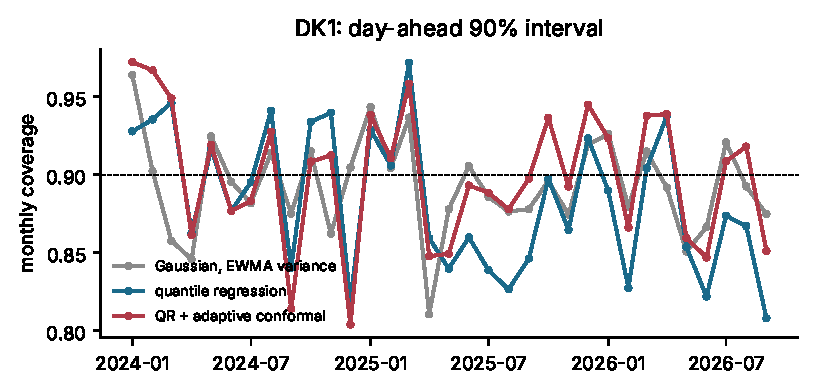
\includegraphics[width=0.49\linewidth]{coverage_DK1.pdf}\hfill
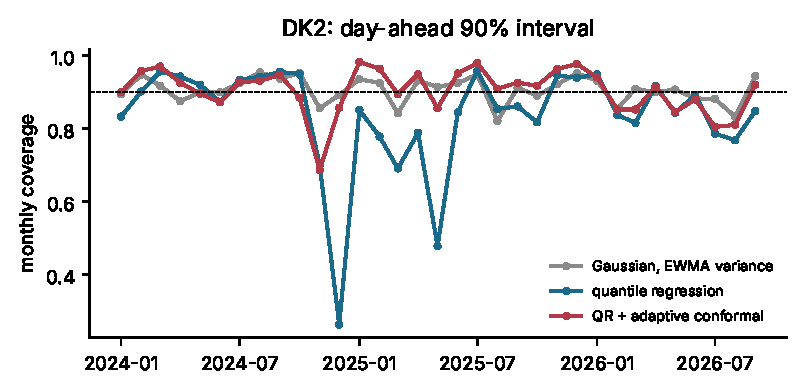
\includegraphics[width=0.49\linewidth]{coverage_DK2.pdf}\\[2pt]
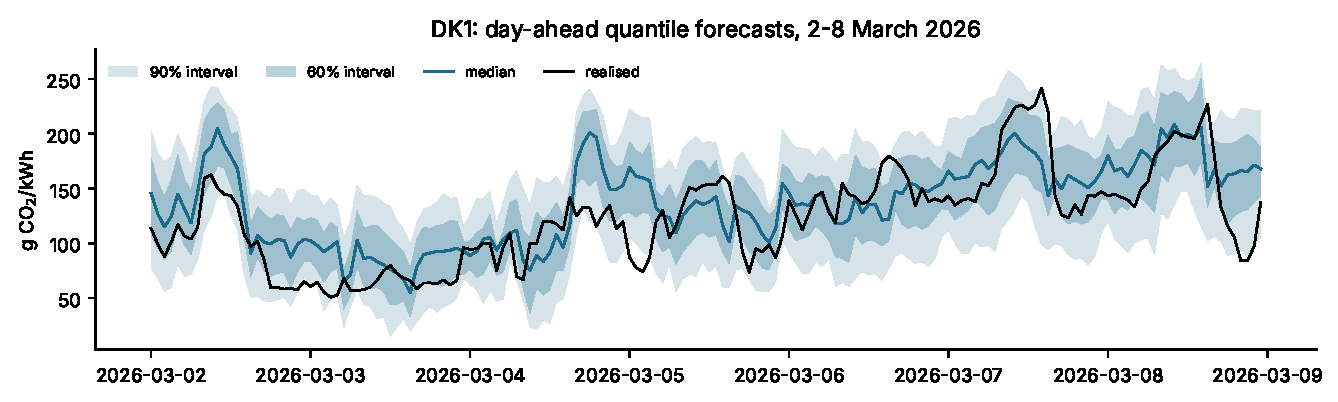
\includegraphics[width=\linewidth]{fan_DK1.pdf}
\caption{Top: monthly coverage of the day-ahead 90\% interval. Bottom: day-ahead quantile forecasts for one week in DK1.}
\label{fig:cov}
\end{figure}

\begin{table}[h]
\centering\small
\caption{Coverage (\%) of the day-ahead 90\% interval by year (2026: January--September).}
\label{tab:covyear}
\begin{tabular}{@{}lccc@{\hspace{1.6em}}ccc@{}}
\toprule
 & \multicolumn{3}{c}{DK1} & \multicolumn{3}{c}{DK2}\\
Year & Gaussian & QR & QR+ACI & Gaussian & QR & QR+ACI\\
\midrule
\csname @@input\endcsname tables/cov_year.tex 
\bottomrule
\end{tabular}
\end{table}

\subsection{Value for a flexible load}
\begin{figure}[t]
\centering
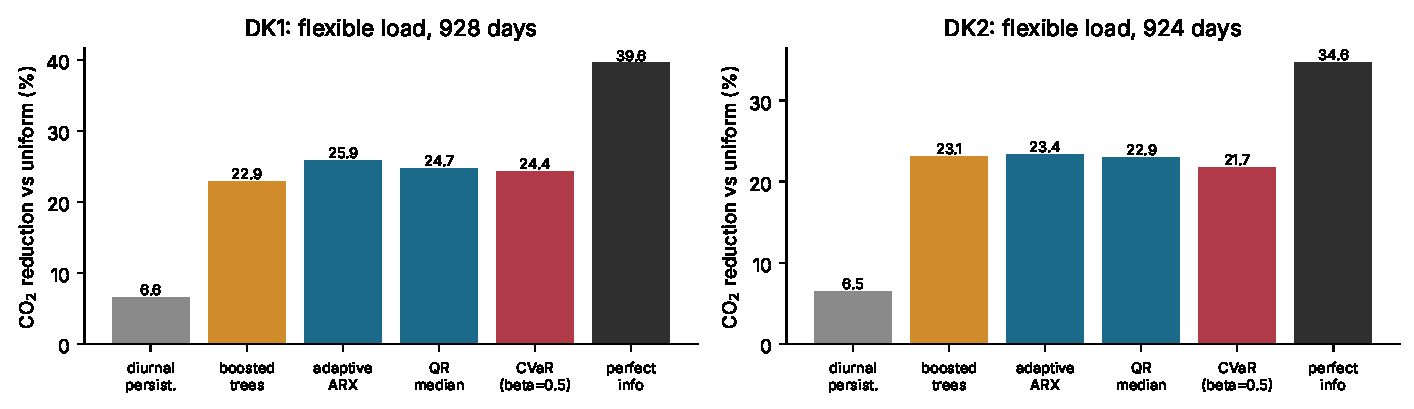
\includegraphics[width=\linewidth]{scheduling_value.pdf}
\caption{Emissions of the flexible energy relative to uniform operation, by the forecast used for scheduling ($E=6$\,MWh/day, $P=1$\,MW).}
\label{fig:sched}
\end{figure}

\begin{table}[h]
\centering\small
\caption{Scheduling results (DK1: \DKabDays{} days, DK2: \DKbbDays{} days). Reduction of emissions of the flexible energy relative to uniform operation, share of the perfect-information reduction, and daily regret relative to perfect information (kg CO$_2$): mean, 95th percentile and the mean of the worst 10\% of days.}
\label{tab:sched}
\begin{tabular}{@{}lcccccc@{\hspace{1.4em}}cc@{}}
\toprule
& \multicolumn{5}{c}{DK1} & & \multicolumn{2}{c}{DK2}\\
\cmidrule(lr){2-6}\cmidrule(lr){8-9}
Forecast used & red.\,\% & share\,\% & regret & p95 & worst 10\% & & red.\,\% & share\,\%\\
\midrule
diurnal persistence & \DKabRedDiur & \DKabShareDiur & \DKabRegMeanDiur & \DKabRegPnfDiur & \DKabRegCvarDiur & & \DKbbRedDiur & \DKbbShareDiur\\
boosted trees & \DKabRedGbm & \DKabShareGbm & \DKabRegMeanGbm & \DKabRegPnfGbm & \DKabRegCvarGbm & & \DKbbRedGbm & \DKbbShareGbm\\
adaptive ARX & \DKabRedRls & \DKabShareRls & \DKabRegMeanRls & \DKabRegPnfRls & \DKabRegCvarRls & & \DKbbRedRls & \DKbbShareRls\\
QR median & \DKabRedQr & \DKabShareQr & \DKabRegMeanQr & \DKabRegPnfQr & \DKabRegCvarQr & & \DKbbRedQr & \DKbbShareQr\\
scenario mean & \DKabRedScen & \DKabShareScen & \DKabRegMeanScen & \DKabRegPnfScen & \DKabRegCvarScen & & \DKbbRedScen & \DKbbShareScen\\
mean--CVaR, $\beta=0.5$ & \DKabRedCvar & \DKabShareCvar & \DKabRegMeanCvar & \DKabRegPnfCvar & \DKabRegCvarCvar & & \DKbbRedCvar & \DKbbShareCvar\\
CVaR, $\beta=1$ & \DKabRedCvarOne & \DKabShareCvarOne & \DKabRegMeanCvarOne & \DKabRegPnfCvarOne & \DKabRegCvarCvarOne & & \DKbbRedCvarOne & \DKbbShareCvarOne\\
perfect information & \DKabRedOracle & 100 & 0 & 0 & 0 & & \DKbbRedOracle & 100\\
\bottomrule
\end{tabular}
\end{table}

Perfect information would cut the emissions of the flexible energy by \DKabRedOracle\% in DK1 and \DKbbRedOracle\% in DK2 (Figure~\ref{fig:sched}, Table~\ref{tab:sched}).
Scheduling on diurnal persistence realises only \DKabShareDiur\% and \DKbbShareDiur\% of that reduction, while the adaptive ARX forecast realises \DKabShareRls\% and \DKbbShareRls\%: the decision value grows much faster than the reduction in MAE, because only the ranking of the hours within a day matters.
The mean--CVaR schedules trade mean for tail performance: with $\beta=0.5$ the 95th percentile of the daily regret falls from \DKabRegPnfRls{} to \DKabRegPnfCvar{} kg in DK1 and from \DKbbRegPnfRls{} to \DKbbRegPnfCvar{} kg in DK2, but the mean reduction drops by one to two percentage points.
For a fixed amount of energy shifted within a day only the ranking of the hours matters, and the errors of different hours are positively correlated (mean correlation of the copula normal scores \DKacopCorr{} in DK1 and \DKbcopCorr{} in DK2), so hedging across hours buys little.
Uncertainty information is likely to matter more for decisions whose cost depends on the level of the intensity, such as a day-ahead flexibility commitment or a carbon budget.

\subsection{Aggregating a heterogeneous fleet}
\begin{figure}[t]
\centering
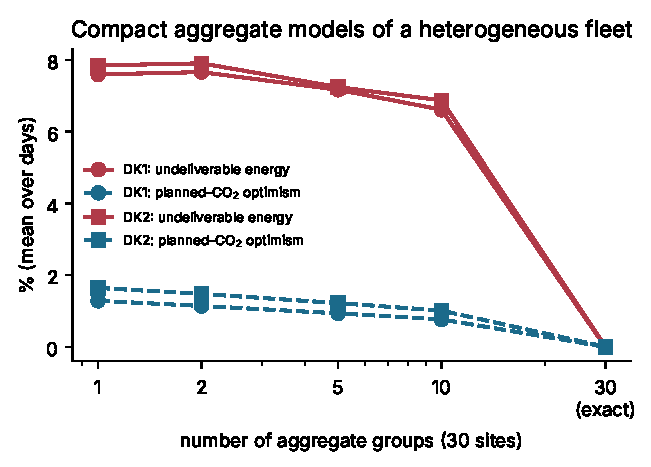
\includegraphics[width=0.6\linewidth]{aggregation.pdf}
\caption{Fleet of 30 sites, day-ahead schedules on the adaptive forecast: energy of the aggregate plan that cannot be delivered by the sites, and the optimism of the planned emissions, against the number of aggregate groups ($k=30$ is exact).}
\label{fig:agg}
\end{figure}
With one envelope for the whole fleet, the planned emissions are only \DKacOptOne\% (DK1) lower than those of the exact fleet schedule, but on each of the \DKacDays{} days part of the aggregate profile cannot be followed by the sites: on average \DKacShortOne\% of the daily energy (maximum \DKacShortMaxOne\%) is left undelivered (DK2: \DKbcShortOne\%).
Clustering sites with similar windows helps only gradually (\DKacShortTen\% with ten groups of three sites, Figure~\ref{fig:agg}): the summed bounds lose the coupling between each site's energy and its own window, and the optimiser concentrates power in exactly the cheap hours where that coupling binds.
A compact flexibility representation for a fleet therefore needs either a disaggregation guarantee (an inner approximation) or a feedback step that corrects the aggregate commitment.

\section{Limitations and next steps}
\begin{itemize}
\item The target is the \emph{average} intensity of consumed electricity under Energinet's accounting; shifting load changes the marginal generator, often abroad \cite{leerbeck2020}, so the emission figures are accounting changes, not system-wide reductions.
\item Release times of the day-ahead inputs are assumed from market practice (Table~\ref{tab:data}); archived values may contain later revisions of the same forecast.
\item The study is hourly; the five-minute horizons needed for real-time balancing, weather inputs, and hierarchical (temporal and spatial) reconciliation \cite{ronlev2026} are natural extensions.
\item The flexible load is a deferrable energy block without thermal dynamics. Cooling flexibility is state dependent and price responsive; describing it with a stochastic flexibility function \cite{junker2018,madsen2025} and aggregating such functions with a disaggregation guarantee is the next question.
\end{itemize}

\paragraph{Reproducibility.} \texttt{python src/data.py} downloads and builds the hourly tables, \texttt{src/run\_forecast.py}, \texttt{src/evaluate.py}, \texttt{src/run\_schedule.py} and \texttt{src/make\_numbers.py} produce every number and figure in this report, and \texttt{python -m unittest discover -s tests} checks the RLS recursion, the absence of look-ahead, the quantile and conformal steps and the scheduling LPs.

\begin{thebibliography}{9}\small
\bibitem{gibbs2021} I.~Gibbs and E.~Cand\`es. Adaptive conformal inference under distribution shift. \emph{NeurIPS}, 2021.
\bibitem{junker2018} R.~G.~Junker et al. Characterizing the energy flexibility of buildings and districts. \emph{Applied Energy}, 225:175--182, 2018.
\bibitem{leerbeck2020} K.~Leerbeck et al. Short-term forecasting of CO$_2$ emission intensity in power grids by machine learning. \emph{Applied Energy}, 277:115527, 2020.
\bibitem{madsen2025} H.~Madsen et al. Recent trends in demand-side flexibility. In \emph{Energy Informatics (EI.A 2024)}, LNCS 15272, Springer, 2025.
\bibitem{pinson2009} P.~Pinson, H.~Madsen, H.~A.~Nielsen, G.~Papaefthymiou and B.~Kl\"ockl. From probabilistic forecasts to statistical scenarios of short-term wind power production. \emph{Wind Energy}, 12(1):51--62, 2009.
\bibitem{rockafellar2000} R.~T.~Rockafellar and S.~Uryasev. Optimization of conditional value-at-risk. \emph{Journal of Risk}, 2(3):21--41, 2000.
\bibitem{ronlev2026} T.~R{\o}nlev-Knudsen, H.~Madsen and J.~K.~M{\o}ller. Online forecast reconciliation using linear models. arXiv:2606.23326, 2026.
\end{thebibliography}
\end{document}
